\section{Durchführung}
\label{sec:Durchführung}

\subsection{Fourier-Analyse}

Bei diesem Versuchsteil werden ein Rechteck-, ein Dreieck- und 
ein Sägezahnsignal in ihre Fourierkomponenten zerlegt. Dazu wird
ein Oszilloskop mit entsprechenden Signalen, die in einem Funktionsgenerator 
erzeugt werden, gespeist, siehe Abbildung \ref{fig:aufbau}. 
Die Fourier-Analyse wird dabei durch das
Oszilloskop durchgeführt und ausgegeben. Zu beachten ist, dass genug
Perioden angezeigt werden müssen, so dass auch genügend Peaks in dem 
Linienspektrum zu sehen sind. Von den angezeigten Peaks werden sowohl
die Frequenz als auch die Amplitude notiert. Wie in der Theorie erwähnt
bilden sich auch Nebenmaxima aus, die hier nicht beachtet werden. 

\begin{figure}
  \centering
  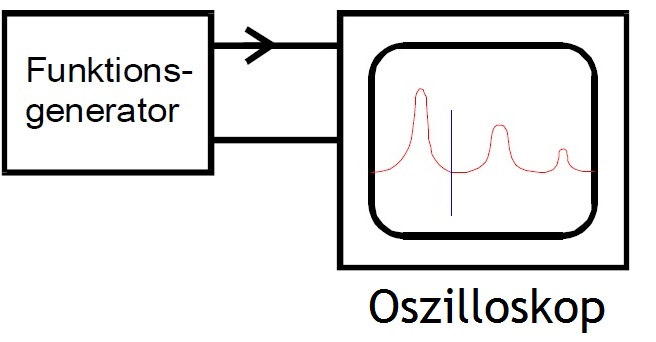
\includegraphics[scale=0.5]{content/Aufbau_1.jpg}
  \caption{Schematischer Aufbau der Messapperatur für die Fourier-Analyse [1].}
  \label{fig:aufbau}
\end{figure}

\subsection{Fourier-Synthese}

Bei der Fourier-Sythese werden Rechtecks-, Dreiecks- und Sägezahnsignal 
aus ihren Fourierkomponenten zusammengesetzt. 
Zunächst werden immer zwei Ausgänge eines Oberwellengenerators an das 
Oszilloskop angeschlossen. Dieser Generator liefert die Oberwellen - von der ersten bis zur n-ten.
Diese sind die Fourierkomponenten. Damit alle Ausgänge 
des Generators in Phase geschaltet sind, wird das Oszilloskop zunächst 
in X-Y-Betrieb geschaltet.
Um eine optimale Genauigkeit zu erreichen, werden die Amplituden der
einzelnenen Oberwellen maximal eingestellt. 
Auf dem Bildschirm erscheint eine Lissajous-Figur, die in sich geschlossen 
oder zu einer Linie mit zwei Enden entartet sein kann. Anhand dieser 
Figur wird die Phase zwischen den beiden Schwingungen bestimmt. Ist die
Figur bei ungeradem $n$ eine Linie, so muss die Phasenverschiebung $\phi$ 
durch 0 oder $\pi$ gegeben sein. Bei geraden $n$ und Sinusfunktion wird
die gleich Phase identifiziert, wenn die Figur eine geschlossene, zur 
x-Achse symmetrische Kurve, ist. Es gibt oft Fälle, bei denen aus der
Gestalt der Lissajous-Figur nicht auf die Phasenverschiebung geschlossen 
werden kann. Ist dies der Fall, wird durch durch Umschalten des 180°-Phasenschalters
während der einzelnen Syntheseschritte die richtige Phaseneinstellung ermittelt. 
Außerdem werden die einzelnen Komponenten gemäß den Beträgen der Fourier-Koeffizienten
eingestellt. Schließlich wird an dem Summenausgang ein Oszilloskop 
angeschlossen und durch sukzessives Zuschalten der einzelnen Komponenten 
die Überlagerungsfigur auf dem Bildschirm beobachtet. 